\paragraph{路径的连接。}\label{sub:concatenation-paths}
设 $\mu_0$、$\mu_1$ 是两条\trMatchingPath，它们只在作为公共端点的一处相遇。我们假定这两条路径的\trOrientation{}取得使 $\mu_0(1)=\mu_1(-1)$（这仅仅是为了方便；在下面的构造中，\trOrientation{}并不起任何作用）。考虑把诸 $\mu_k$ 连接起来、再把它们移到公共端点右侧而得的路径 $\mu=\mu_1\#\mu_0$（\cref{fig:path-concatenation}；这是一个非对称的运算，取决于我们给这两条路径排定的先后）。十分明显，$\mu$ 仍是一条\trMatchingPath。我们想要解释的结果是说：相伴的\trMatchingCycle{}$\Sigma_\mu$ 可由 $\Sigma_{\mu_0}$ 沿 $\Sigma_{\mu_1}$ 作\trDehnTwist{}而得到。为把这个陈述说得更精确，还需要把\trFrame{}与\trIsotopy{}纳入考量。每个 $\mu_k$ 都\trSplitting{}成一对\trVanishingPath{}$\gamma_k^\pm$，于是共有四个相伴的\trVanishingCycle。为方便计，不妨假定 $\mu|[-1;-1/2]$ 在显然的重新\trParametrization{}之下与 $\mu_0|[-1;0]$ 一致，$\mu|[1/2;1]$ 同样与 $\mu_1|[0;1]$ 一致。连接而成的路径 $(\mu|[-1/2;0])^{-1}\cdot\gamma_0^+$ 与 $(\mu|[0;1/2])\cdot\gamma_1^-$ 相对于端点\trHomotopic；由此在 $E_{\mu(0)}$%
\footnote{译注：原书此处印作 $E_{\mu_1(0)}$；疑应为 $E_{\mu(0)}$（按本页自证的 $h_\gamma\colon E_{\gamma(0)}\to E_{\gamma(1)}$ 约定及 \eqref{eq:split-vanishing-isotopy} 两端所在\trFiber{}，该带\trFrame{}\trIsotopy{}应居于 $E_{\mu(0)}$，而 $E_{\mu_1(0)}=E_{\mu(1/2)}$ 并非其所在\trFiber{}）；此处径改。——译者注}
中得到一个带\trFrame{}的\trIsotopy：
\begin{equation}\label{eq:split-vanishing-isotopy}
h_{\mu|[-1/2;0]}(V_{\gamma_0^+})\simeq h_{\mu|[0;1/2]}^{-1}(V_{\gamma_1^-}).
\end{equation}
按需选取\trIsotopy{}$I_k$，以定义诸\trMatchingCycle{}$\Sigma_{\mu_k,I_k}$。与\eqref{eq:split-vanishing-isotopy}相结合，这些便给出一个介于 $\mu$ 的两半 $\gamma^\pm$ 的\trVanishingCycle{}之间的\trIsotopy{}$I$：
\begin{equation*}
V_{\gamma^-}=h_{\mu|[-1/2;0]}(V_{\gamma_0^-})\overset{I}{\simeq}h_{\mu|[0;1/2]}^{-1}(V_{\gamma_1^+})=V_{\gamma^+},
\end{equation*}
而我们用它来定义另一个\trMatchingCycle{}$\Sigma_{\mu,I}$。
\begin{figure}[htbp]
\centering
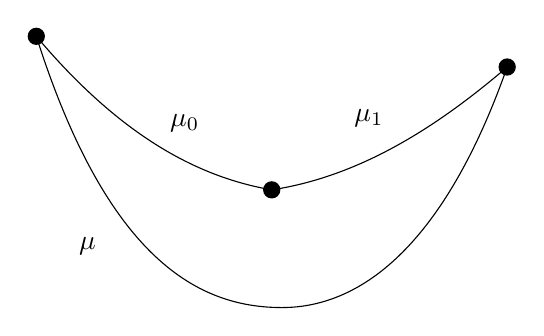
\begin{tikzpicture}[line cap=round,line join=round,scale=1.3]
\fill (-2.3,1.7) circle (2.4pt);%
\fill (2.3,1.4) circle (2.4pt);%
\fill (0,0.2) circle (2.4pt);%
\draw (-2.3,1.7) .. controls (-1.5,0.75) and (-0.75,0.33) .. (0,0.2);
\draw (0,0.2) .. controls (0.85,0.33) and (1.6,0.8) .. (2.3,1.4);
\draw (-2.3,1.7) .. controls (-1.6,-0.5) and (-0.7,-0.95) .. (0.1,-0.95)
      .. controls (0.9,-0.95) and (1.7,-0.3) .. (2.3,1.4);
\node at (-0.85,0.85) {$\mu_0$};
\node at (0.95,0.9) {$\mu_1$};
\node at (-1.8,-0.35) {$\mu$};
\end{tikzpicture}
\caption{}\label{fig:path-concatenation}
\end{figure}
\begin{lemma}\label{thm:matching-concatenation-twist}
$E$ 中存在一个由带\trFrame{}的\trLagrange\trSphere{}构成的\trIsotopy，
\begin{equation}\label{eq:matching-cycle-twist}
\Sigma_{\mu,I}\simeq\tau_{\Sigma_{\mu_1,I_1}}(\Sigma_{\mu_0,I_0}).
\end{equation}
\end{lemma}
\begin{proof}
这是经由\trDeformation{}归约到较简单特殊情形的一个典型论证。若该结果对某个\trExact\trLefschetzFibration{}成立，那么它对这一\trFibration{}的任何\trDeformation{}（沿 $\partial^hE$ \trWellBehaved{}的\trDeformation{}之义）也成立；这是因为，一旦对\trDeformation{}后的\trLefschetzFibration{}结构找到了一个\trIsotopy，便可以把它与一族如\cref{thm:moser-deformation-embedding}中的\trConformallySymplectic{}\trEmbedding{}相结合，从而对原先的结构得到一个\trIsotopy。鉴于\cref{thm:transport-isotopy-realization}与证明\trPicard--\trLefschetz{}公式时所用的技巧，因此容许作出如下假定：与 $\mu_0$ 的两半相关联的那对\trVanishingCycle{}彼此重合，对 $\mu_1$ 亦然；\trIsotopy{}$I_0$、$I_1$ 都是常值的；并且在 $E_{\mu_0(1)}$ 中那个唯一的\trCriticalPoint{}附近，存在\trHolomorphic{}坐标，使 $\pi$ 在其中成为标准的\trQuadraticForm{}\eqref{eq:standard-quadratic-map}，而 $\omega_E$ 成为 $\CC^{n+1}$ 上的标准\trKaehler{}形式。再者，仍不影响陈述地，我们可以把所涉路径\trDeformation，使得：在 $\mu_0(1)$ 附近的局部坐标中，$\mu_0$ 与 $\mu_1$ 分别是负实半轴与正实半轴；而 $\mu$ 在该点的一个小邻域之外与 $\mu_0\cup\mu_1$ 一致。于是，在 $E_{\mu_0(1)}$\footnote{译注：原书此处印作 $E_{\mu_1(1)}$；疑应为 $E_{\mu_0(1)}$（即 $E_{\mu_1(-1)}$——全\trFibration{}唯一的\trCriticalPoint{}落在公共\trCriticalValue{}$\mu_0(1)=\mu_1(-1)$ 之上的\trFiber{}中，同段前文亦作 $E_{\mu_0(1)}$，而 $E_{\mu_1(1)}$ 是\trRegular\trFiber、不含\trCriticalPoint）；此处径改。——译者注}中该\trCriticalPoint{}的一个小邻域之外，有 $\Sigma_{\mu,I}=\Sigma_{\mu_0,I_0}\cup\Sigma_{\mu_1,I_1}$；而在该点附近，我们有下面的局部图景，它来自\cref{thm:toy-model-thimble}：
\begin{equation}\label{eq:lagrangian-handle-picture}
\Sigma_{\mu_0,I_0}=i\RR^{n+1},\qquad
\Sigma_{\mu_1,I_1}=\RR^{n+1},\qquad
\Sigma_{\mu,I}=\bigcup_t\sqrt{\mu(t)}\,S^n
\end{equation}
其中 $\sqrt{\mu}$ 是 $\CC$ 中一条位于闭右下象限内的\trSmooth\trEmbedding{}路径，它使得当 $t<-\epsilon$ 时 $\sqrt{\mu(t)}=it$，当 $t>\epsilon$ 时 $\sqrt{\mu(t)}=t$，这里 $\epsilon$ 是某个较小的数。\eqref{eq:lagrangian-handle-picture} 中的第三个\trSubmanifold{}就是\textbf{\trLagrange\trHandle}（Lagrangian handle），它出现于\trLagrange\trConnectedSum{}或\trLagrange{}手术的构造之中。把那种和同样记作 $\#$，并采用 [125, Section 2e] 的约定，便有
\begin{equation}\label{eq:matching-connected-sum}
\Sigma_{\mu,I}=\Sigma_{\mu_1,I_1}\#\Sigma_{\mu_0,I_0}.
\end{equation}
但 \eqref{eq:matching-cycle-twist} 与 \eqref{eq:matching-connected-sum} 的右边在相差\trLagrange\trIsotopy{}的意义下是相同的 [124, Appendix]。诸\trIsotopy{}$I_0$、$I_1$ 与 $I$ 都是常值的，故容易验证这一点与\trFrame{}\trCompatible。
\end{proof}
\begin{remark}\label{thm:matching-half-sum-remark}
既然已经采用了记号 $\mu=\mu_1\#\mu_0$，\eqref{eq:matching-cycle-twist} 便可以写得更直观一些（把\trHomotopy{}置之不计）：$\Sigma_{\mu_1\#\mu_0}=\Sigma_{\mu_1}\#\Sigma_{\mu_0}$。此外还有一种重要的解释。也就是说，设 $t_{\mu_1}$ 是沿 $\mu_1$ 的\trHalfTwist。由于 $\mu$ \trIsotopy{}于 $t_{\mu_1}(\mu_0)$，我们所证明的便是
\begin{equation*}
\Sigma_{t_{\mu_1}(\mu_0)}\simeq\tau_{\Sigma_{\mu_1}}(\Sigma_{\mu_0}).
\end{equation*}
在这一形式下，该陈述可推广到任意相交的\trMatchingPath{}$\mu_0$、$\mu_1$。然而，其证明与上面处理的特殊情形颇为不同，我们在此不予给出，因为我们对它并无实际需要（不过请注意，引理 18.3 可视为另一个特殊情形）。
\end{remark}
